\documentclass{article}
\usepackage[mast]{lucky}

\title{Solutions to Basics of Geometry}
\author{Dennis Chen}
\date{GPV1}

\begin{document}
\maketitle

\toc

\pagebreak\section{AMC 10A 2020/12}
Triangle $AMC$ is isosceles with $AM = AC$. Medians $\overline{MV}$ and $\overline{CU}$ are perpendicular to each other, and $MV=CU=12$. What is the area of $\triangle AMC?$

\begin{center}
\begin{asy}
import olympiad;
size(4cm);
draw((-4,0)--(4,0)--(0,12)--cycle);
draw((-2,6)--(4,0));
draw((2,6)--(-4,0));
label("M", (-4,0), W);
label("C", (4,0), E);
label("A", (0, 12), N);
label("V", (2, 6), NE);
label("U", (-2, 6), NW);
label("P", (0, 3.6), S);
\end{asy}
\end{center}

\subsection{Solution}

Because the centroid splits the median in a $2$ to $1$ ratio, $PM=PC=8.$ Also note that the height from $P$ to $MC$ is $\frac{1}{3}$ of the height from $A$ to $MC,$ so $[AMC]=3[PMC].$ Also note that $[PMC]=\frac{8\cdot 8}{2}=32,$ so $[AMC]=96.$

\pagebreak\section{Brazil 3rd Phase Level 2 2004/1}

In the figure, $ABC$ and $DAE$ are isosceles triangles ($AB = AC = AD = DE$) and the angles $BAC$ and $ADE$ have measures $36^{\circ}$.
\begin{enumerate}
    \item Using geometric properties, calculate the measure of angle $\angle EDC$.
    \item Knowing that $BC = 2$, calculate the length of segment $DC$.
    \item Calculate the length of segment $AC$.
\end{enumerate}
\begin{center}
\begin{asy}
import olympiad;
size(4cm);
pair A=(0,0),B=dir(0),C=dir(36),D=dir(72),E=(2cos(0.4pi),0);
dot(A^^B^^C^^D^^E);
draw(A--B--C--cycle);
draw(A--D--E);
draw(D--C,dotted);
label("A",A,dir(-90));
label("B",B,dir(-90));
label("C",C,dir(40));
label("D",D,dir(90));
label("E",E,dir(-90));
\end{asy}
\end{center}

\subsection{Solution}

The main idea is expressing angles in terms of differences of other angles.
\begin{enumerate}
\item Note that $\angle DAC=\angle DAE-\angle CAB=72^{\circ}-36^{\circ}=36^{\circ},$ and also note that $\angle EDC=\angle ADC-\angle ADE=72^{\circ}-36^{\circ}=36^{\circ}.$

\item Note that $\angle DAC=\angle CAB$ from our progress on the first part, so $DC=BC=2.$

\item By the Law of Sines, $\frac{AC}{DC}=\frac{AC}{2}=\frac{\sin 72^{\circ}}{\sin 36^{\circ}}=\frac{2\sin 36^{\circ}\cos 36^{\circ}}{\sin 36^{\circ}}=2\cos 36^{\circ},$ so $AC=4\cos 36^{\circ}=\sqrt{5}+1.$
\end{enumerate}

\pagebreak\section{Unsourced}

Let circles $\omega_1$ and $\omega_2$ intersect at $X,Y.$ Let line $\ell_1$ passing through $X$ intersect $\omega_1$ at $A$ and $\omega_2$ at $C,$ and let line $\ell_2$ passing through $Y$ intersect $\omega_1$ at $B$ and $\omega_2$ at $D.$ If $\ell_1$ intersects $\ell_2$ at $P,$ prove that $\triangle PAB\sim \triangle PCD.$

\subsection{Solution}

We only prove it for the configuration below. We can use directed angles or casework to take care of all configurations.

We want to prove that $\angle PAB=\angle PCD.$ Note that
\[\angle PCD=\angle 180^{\circ}-\angle XCD=\angle XYD=180^{\circ}-\angle XYB=\angle XAB=\angle PAB.\]

\begin{center}
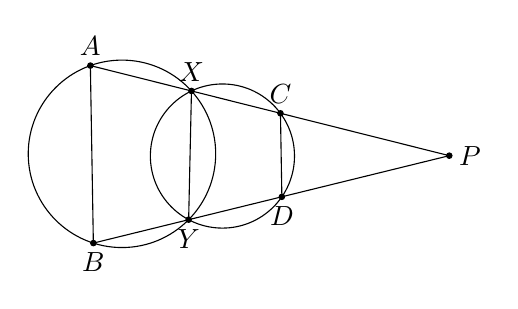
\begin{tikzpicture}[scale=0.7]
\draw (0.4787341389728096,3.099439577039275) circle (1.7004910028038982cm);
\draw (2.3017280966767366,3.0593927492447124) circle (1.3074295144029862cm);
\draw (-0.09435730463284764,4.700450460163744)-- (6.417150824513995,3.0659668691788755);
\draw (6.417150824513995,3.0659668691788755)-- (-0.04,1.48);
\draw (-0.04,1.48)-- (-0.09435730463284764,4.700450460163744);
\draw (3.3544327897751343,3.834753803374101)-- (3.38,2.32);
\draw (1.74,4.24)-- (1.688696661828737,1.9045921625544264);

\filldraw (-0.04,1.48) circle (1.4pt) node[anchor=north]{$B$};
\filldraw (3.38,2.32) circle (1.4pt) node[anchor=north]{$D$};
\filldraw (1.688696661828737,1.9045921625544264) circle (1.4pt) node[anchor=north]{$Y$};
\filldraw (1.74,4.24) circle (1.4pt) node[anchor=south]{$X$};
\filldraw (-0.09435730463284764,4.700450460163744) circle (1.4pt) node[anchor=south]{$A$};
\filldraw (3.3544327897751343,3.834753803374101) circle (1.4pt) node[anchor=south]{$C$};
\filldraw (6.417150824513995,3.0659668691788755) circle (1.4pt) node[anchor=west]{$P$};
\end{tikzpicture}
\end{center}

\pagebreak\section{AMC 10B 2011/17}

In the given circle, the diameter $\overline{EB}$ is parallel to $\overline{DC}$, and $\overline{AB}$ is parallel to $\overline{ED}$. The angles $AEB$ and $ABE$ are in the ratio $4 : 5$. What is the degree measure of angle $BCD?$

\begin{center}
\begin{asy}
import olympiad;

size(4cm);

real r=3;
pair A=(-3cos(80),-3sin(80));
pair D=(3cos(80),3sin(80)), C=(-3cos(80),3sin(80));
pair O=(0,0), E=(-3,0), B=(3,0);
path outer=Circle(O,r);
draw(outer);
draw(E--B);
draw(E--A);
draw(B--A);
draw(E--D);
draw(C--D);
draw(B--C);

pair[] ps={A,B,C,D,E,O};
dot(ps);

label("$A$",A,N);
label("$B$",B,NE);
label("$C$",C,S);
label("$D$",D,S);
label("$E$",E,NW);
\end{asy}
\end{center}

\subsection{Solution}

Note that $\angle EAB=90^{\circ},$ as $AB$ is a diameter. Thus $\angle AEB=40^{\circ}$ and $\angle ABE=50^{\circ}.$ Since $AB$ and $DE$ are parallel, the measures of the arcs must be the same, so $\angle BED=50^{\circ}.$ By the cyclic quadrilateral criterion, $\angle BCD=180^{\circ}-\angle BED=130^{\circ}.$

Note that the fact that $DC$ is parallel to $EB$ is irrelevant, other than determining the configuration.

\pagebreak\section{Dennis Chen}

Consider rectangle $ABCD$ with $AB = 6,$ $BC = 8.$ Let $M$ be the midpoint of $AD$ and let $N$ be the midpoint of $CD.$ Let $BM$ and $BN$ intersect $AC$ at $X$ and $Y$ respectively. Find $XY.$

\subsection{Solution}

Let $BD$ intersect $AC$ and $MN$ at $P$ and $Q,$ respectively. Note that $\triangle BXY\sim \triangle BMN,$ and also note that the similarity taking $\triangle BXY$ to $\triangle BMN$ also takes $P$ to $Q.$ Since $BP=\frac{2}{3}BQ,$ $XY=\frac{2}{3}MN=\frac{10}{3}.$

\begin{center}
\begin{tikzpicture}[scale=0.4]
\coordinate (A) at (0,6);
\coordinate (B) at (0,0);
\coordinate (C) at (8,0);
\coordinate (D) at (8,6);

\coordinate (M) at ($1/2*(A)+1/2*(D)$);
\coordinate (N) at ($1/2*(C)+1/2*(D)$);

\coordinate (X) at ($1/3*(A)+1/3*(B)+1/3*(D)$);
\coordinate (Y) at ($1/3*(C)+1/3*(B)+1/3*(D)$);

\coordinate (P) at ($1/2*(A)+1/2*(C)$);
\coordinate (Q) at ($1/2*(M)+1/2*(N)$);

\draw (A)--(B)--(C)--(D)--cycle;
\draw (M)--(B)--(N);
\draw[dotted] (M)--(N);
\draw[dotted] (B)--(D);
\draw (A)--(C);

\filldraw (A) circle (1.4pt) node[anchor=south]{$A$};
\filldraw (B) circle (1.4pt) node[anchor=north]{$B$};
\filldraw (C) circle (1.4pt) node[anchor=north]{$C$};
\filldraw (D) circle (1.4pt) node[anchor=south]{$D$};

\filldraw (M) circle (1.4pt) node[anchor=south]{$M$};
\filldraw (N) circle (1.4pt) node[anchor=west]{$N$};

\filldraw (P) circle (1.4pt) node[anchor=south]{$P$};
\filldraw (Q) circle (1.4pt) node[anchor=south]{$Q$};

\filldraw (X) circle (1.4pt) node[anchor=south]{$X$};
\filldraw (Y) circle (1.4pt) node[anchor=south]{$Y$};
\end{tikzpicture}
\end{center}

\pagebreak\section{AMC 10A 2019/13}

Let $\triangle ABC$ be an isosceles triangle with $BC = AC$ and $\angle ACB = 40^{\circ}$. Construct the circle with diameter $\overline{BC}$, and let $D$ and $E$ be the other intersection points of the circle with the sides $\overline{AC}$ and $\overline{AB}$, respectively. Let $F$ be the intersection of the diagonals of the quadrilateral $BCDE$. What is the degree measure of $\angle BFC?$

\subsection{Solution}

Notice that $\angle BFC=\angle DFE.$ Now note that $\angle BEC=\angle BDC=90^{\circ},$ so $CE$ and $BD$ are altitudes. Now note that $\angle FEA=\angle FDA=90^{\circ},$ so $FEAD$ is also cyclic. Thus $\angle DFE=180^{\circ}-\angle DAE=110^{\circ}.$

\begin{center}
\begin{asy}
size(4cm);
draw((-1,0)--(1,0)--(0,2.75)--cycle);draw(circumcircle((-1,0),(0,0),(0,2.75)));label("$A$",(1,0),SE);label("$C$",(0,2.75),N);label("$B$",(-1,0),SW);label("$E$",(0,0),S);label("$D$",(0.77,0.64),E);draw((0,0)--(0,2.75));draw((-1,0)--(0.77,0.64));
draw(circumcircle((1,0),(0,0),(0.766,0.642)),dotted);
label("$F$",(0,4/11),NW);
\end{asy}
\end{center}

\pagebreak\section{Miquel's Theorem}

Consider $\triangle ABC$ with $D$ on $BC,$ $E$ on $CA,$ and $F$ on $AB.$ Prove that $(AEF),$ $(BFD),$ and $(CDE)$ concur.

\subsection{Solution}

We only prove the case where $D,E,F$ are on segments $BC,CA,AB.$ The other configurations can be proved with directed angles.

Let $(AEF)$ and $(BFD)$ intersect at $P.$ We then prove that $P$ lies on $(CED).$ Note that
\[\angle DPE=360^{\circ}-\angle EPF-\angle FPD=360^{\circ}-(180^{\circ}-\angle A)-(180^{\circ}-\angle B)=\angle A+\angle B.\]
Since $\angle A+\angle DPE=180^{\circ},$ $(CDPE)$ is cyclic.

\begin{center}
\begin{tikzpicture}[scale=0.8]
\coordinate (A) at (0,0);
\coordinate (B) at (4,0);
\coordinate (C) at (1,3);

\coordinate (D) at ($1/2*(B)+1/2*(C)$);
\coordinate (E) at ($1/2*(C)+1/2*(A)$);
\coordinate (F) at ($1/2*(A)+1/2*(B)$);

\draw(A)--(B)--(C)--cycle;

\tkzDefCircle[circum](E,F,A)
\tkzGetPoint{O} \tkzGetLength{rayon}
\tkzDrawCircle[R](O,\rayon pt)

\tkzDefCircle[circum](F,D,B)
\tkzGetPoint{O} \tkzGetLength{rayon}
\tkzDrawCircle[R](O,\rayon pt)

\tkzDefCircle[circum](D,E,C)
\tkzGetPoint{O} \tkzGetLength{rayon}
\tkzDrawCircle[R,dotted](O,\rayon pt)

\tkzDefCircle[circum](A,B,C)
\tkzGetPoint{O} \tkzGetLength{rayon}
\filldraw (O) circle (1.4pt) node[anchor=south]{$P$};

\filldraw (A) circle (1.4pt) node[anchor=east]{$A$};
\filldraw (B) circle (1.4pt) node[anchor=west]{$B$};
\filldraw (C) circle (1.4pt) node[anchor=south]{$C$};
\filldraw (D) circle (1.4pt) node[anchor=south]{$D$};
\filldraw (E) circle (1.4pt) node[anchor=east]{$E$};
\filldraw (F) circle (1.4pt) node[anchor=north]{$F$};
\end{tikzpicture}
\end{center}

\pagebreak\section{Unsourced}

Consider $\triangle ABC$ with $D$ on segment $BC,$ $E$ on segment $CA,$ and $F$ on segment $AB.$ Let the circumcircles of $\triangle FBD$ and $\triangle DCE$ intersect at $P\neq D.$ If $\angle A=50^{\circ},\angle B=35^{\circ},$ find $\angle DPE.$

\subsection{Solution}

By Miquel's Theorem, $(CDPE)$ is cyclic, so $\angle DPE=180^{\circ}-\angle C=85^{\circ}.$

\begin{center}
\begin{tikzpicture}[scale=0.8]
\coordinate (A) at (0,0);
\coordinate (B) at (4,0);
\coordinate (C) at (1,3);

\coordinate (D) at ($1/2*(B)+1/2*(C)$);
\coordinate (E) at ($1/2*(C)+1/2*(A)$);
\coordinate (F) at ($1/2*(A)+1/2*(B)$);

\draw(A)--(B)--(C)--cycle;

\tkzDefCircle[circum](E,F,A)
\tkzGetPoint{O} \tkzGetLength{rayon}
\tkzDrawCircle[R](O,\rayon pt)

\tkzDefCircle[circum](F,D,B)
\tkzGetPoint{O} \tkzGetLength{rayon}
\tkzDrawCircle[R](O,\rayon pt)

\tkzDefCircle[circum](D,E,C)
\tkzGetPoint{O} \tkzGetLength{rayon}
\tkzDrawCircle[R,dotted](O,\rayon pt)

\tkzDefCircle[circum](A,B,C)
\tkzGetPoint{O} \tkzGetLength{rayon}
\filldraw (O) circle (1.4pt) node[anchor=south]{$P$};

\filldraw (A) circle (1.4pt) node[anchor=east]{$A$};
\filldraw (B) circle (1.4pt) node[anchor=west]{$B$};
\filldraw (C) circle (1.4pt) node[anchor=south]{$C$};
\filldraw (D) circle (1.4pt) node[anchor=south]{$D$};
\filldraw (E) circle (1.4pt) node[anchor=east]{$E$};
\filldraw (F) circle (1.4pt) node[anchor=north]{$F$};
\end{tikzpicture}
\end{center}

\pagebreak\section{AIME II 2018/4}

In equiangular octagon $CAROLINE$, $CA = RO = LI = NE =$ $\sqrt{2}$ and $AR = OL = IN = EC = 1$. The self-intersecting octagon $CORNELIA$ encloses six non-overlapping triangular regions. Let $K$ be the area enclosed by $CORNELIA$, that is, the total area of the six triangular regions. Then $K =$ $\dfrac{a}{b}$, where $a$ and $b$ are relatively prime positive integers. Find $a + b$.

\subsection{Solution}

Say that the center of $CAROLINE$ is $M,$ and let $MA$ and $MR$ intersect $CO$ at $W$ and $X,$ and let $MI$ and $MN$ intersect $LE$ at $Y$ and $Z.$

By similar triangles, $WX=\frac{AR}{3}=\frac{1}{3},$ so $[MWX]=\frac{1}{2}\cdot (\frac{1}{3}\cdot \frac{1}{2})=\frac{1}{12}.$ This implies that $CW=\frac{CO-WX}{2}=\frac{3-\frac{1}{3}}{2}=\frac{4}{3},$ so $[CAW]=\frac{1}{2}\cdot (\frac{4}{3}\cdot 1)=\frac{2}{3}.$ Now note
\[[CORNELIA]=4[CAW]+2[WMX]=4\cdot \frac{2}{3}+2\cdot\frac{1}{12}=\frac{17}{6},\]
so the answer is $17+6=23.$

\begin{center}
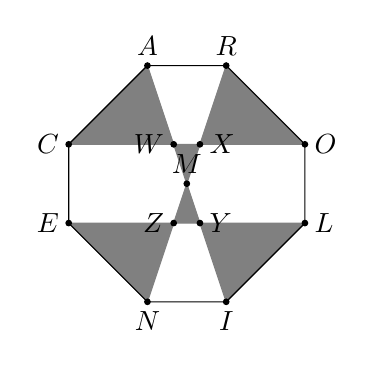
\begin{tikzpicture}
\filldraw[color=gray] (0,2)--(3,2)--(2,3)--(1,0)--(0,1)--(3,1)--(2,0)--(1,3)--cycle;

\draw (1,0)--(2,0)--(3,1)--(3,2)--(2,3)--(1,3)--(0,2)--(0,1)--cycle;

\filldraw (0,2) circle(1pt) node[anchor=east]{$C$};
\filldraw (1,3) circle(1pt) node[anchor=south]{$A$};
\filldraw (2,3) circle(1pt) node[anchor=south]{$R$};
\filldraw (3,2) circle(1pt) node[anchor=west]{$O$};
\filldraw (3,1) circle(1pt) node[anchor=west]{$L$};
\filldraw (2,0) circle(1pt) node[anchor=north]{$I$};
\filldraw (1,0) circle(1pt) node[anchor=north]{$N$};
\filldraw (0,1) circle(1pt) node[anchor=east]{$E$};

\filldraw (4/3,2) circle(1pt) node[anchor=east]{$W$};
\filldraw (5/3,2) circle(1pt) node[anchor=west]{$X$};
\filldraw (4/3,1) circle(1pt) node[anchor=east]{$Z$};
\filldraw (5/3,1) circle(1pt) node[anchor=west]{$Y$};

\filldraw (1.5,1.5) circle(1pt) node[anchor=south]{$M$};
\end{tikzpicture}
\end{center}

\pagebreak\section{Brazil 3rd Phase Level 2 2007/1}

Let $ABC$ be a triangle with circumcenter $O$. Let $P$ be the intersection of straight lines $BO$ and $AC$ and $\omega$ be the circumcircle of triangle $AOP$. Suppose that $BO = AP$ and that the measure of the arc $OP$ in $\omega$, that does not contain $A$, is $40^{\circ}$. Determine the measure of the angle $\angle OBC$.

\subsection{Solution}

Note that $BO=AO=AP,$ so $\triangle AOP$ is isosceles. Thus $\angle OAP=20^{\circ},$ implying $\angle AOC=140^{\circ},$ and $\angle AOP=\angle APO=80^{\circ},$ implying that $\angle AOB=100^{\circ}.$ So $\angle OBC=360^{\circ}-140^{\circ}-100^{\circ}=120^{\circ},$ or $\angle OBC=30^{\circ}.$
    
    \begin{center}
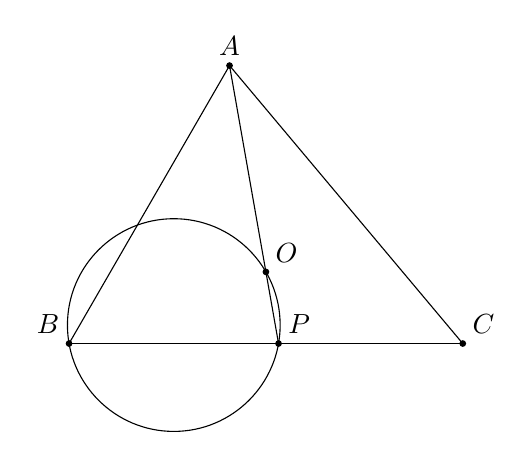
\begin{tikzpicture}
\draw (0.,0.)-- (5.,0.);
\draw (2.038018672739762,3.529951887959356)-- (0.,0.);
\draw (2.660444431189779,0.)-- (2.038018672739762,3.529951887959356);
\draw (2.038018672739762,3.529951887959356)-- (5.,0.);
\draw (1.3302222155948895,0.23455406694717237) circle (1.3507430374366678cm);

\filldraw (0.,0.) circle (1pt) node[anchor=south east] {$B$};
\filldraw (5.,0.) circle (1pt) node[anchor=south west] {$C$};
\filldraw (2.038018672739762,3.529951887959356) circle (1pt) node[anchor=south] {$A$};
\filldraw (2.5,0.9099255856655059) circle (1pt) node[anchor=south west] {$O$};
\filldraw (2.660444431189779,0.) circle (1pt) node[anchor=south west] {$P$};
\end{tikzpicture}
    \end{center}

\pagebreak\section{Unsourced}

Consider square $ABCD$ and some point $P$ outside $ABCD$ such that $\angle APB=90^{\circ}.$ Prove that the angle bisector of $\angle APB$ also bisects the area of $ABCD.$

\subsection{Solution}

Let $Q,R,S$ be the rotations of $P$ about $O$ by $90^{\circ},180^{\circ},270^{\circ}$ counterclockwise. Note that $PR$ is the angle bisector of $\angle APB$ and $PR$ bisects the area of $[PQRS].$ Since the area we added to both halves of $ABCD$ is the same, $PR$ also bisects $ABCD.$

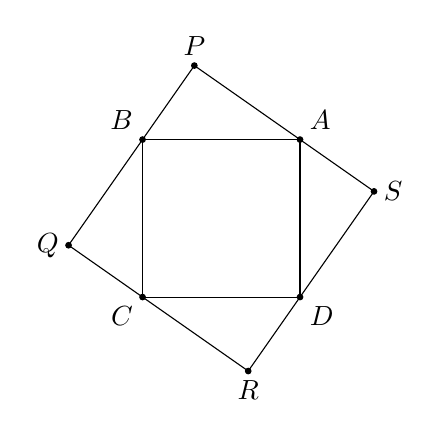
\begin{tikzpicture}
    \draw (-1,-1)--(-1,1)--(1,1)--(1,-1)--cycle;
    \filldraw (-1,-1) circle (1pt) node[anchor=north east] {$C$};
    \filldraw (-1,1) circle (1pt) node[anchor=south east] {$B$};
    \filldraw (1,1) circle (1pt) node[anchor=south west] {$A$};
    \filldraw (1,-1) circle (1pt) node[anchor=north west] {$D$};
    
    \draw (-0.342020143,1.93969262)--(1.93969262,0.342020143)--(0.342020143,-1.93969262)--(-1.93969262,-0.342020143)--cycle;
    \filldraw (-0.342020143,1.93969262) circle (1pt) node[anchor=south] {$P$};
    \filldraw (1.93969262,0.342020143) circle (1pt) node[anchor=west] {$S$};
    \filldraw (0.342020143,-1.93969262) circle (1pt) node[anchor=north] {$R$};
    \filldraw (-1.93969262,-0.342020143) circle (1pt) node[anchor=east] {$Q$};
    \end{tikzpicture}

\pagebreak\section{AMC 10B 2018/12}

Line segment $\overline{AB}$ is a diameter of a circle with $AB=24$. Point $C$, not equal to $A$ or $B$, lies on the circle. As point $C$ moves around the circle, the centroid (center of mass) of $\triangle{ABC}$ traces out a closed curve missing two points. To the nearest positive integer, what is the area of the region bounded by this curve?

\subsection{Solution}

Let $O$ be the center of the circle and $G$ be the centroid of $\triangle ABC.$ Since $O$ is also the midpoint of $AB$ and thus lies on $CG$, we're motivated to make use of the $2:1$ ratio. $CO$ always has length $12,$ so it follows that $GO$ always has length $4.$ This means that the locus of $G$ is a circle with center $O$ and radius $4$ by definition, so the area is $16\pi\approx 50.$

\begin{center}
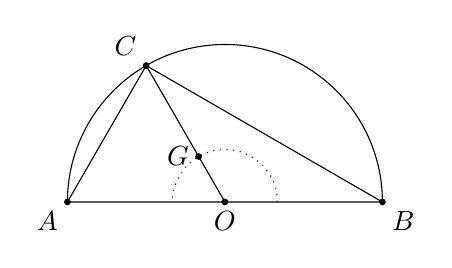
\begin{tikzpicture}
\draw (0,0)--(4,0)--(1,1.73205081)--cycle;
\draw (1,1.73205081)--(2,0);
\filldraw (0,0) circle (1pt) node[anchor= north east] {$A$};
\filldraw (4,0) circle (1pt) node[anchor=north west] {$B$};
\filldraw (1,1.73205081) circle (1pt) node[anchor=south east] {$C$};
\filldraw (2,0) circle (1pt) node[anchor= north] {$O$};
\filldraw (1.66666,0.57735027) circle (1pt) node[anchor= east] {$G$};
\draw (4,0) arc (0:180:2);
\draw[dotted] (8/3,0) arc (0:180:2/3);
\end{tikzpicture}
\end{center}

\pagebreak\section{Formula of Unity Qualifying Round Grade 11 2018/4}

A point $O$ is the center of an equilateral triangle $ABC.$ A circle that passes through points $A$ and $O$ intersects the sides $AB$ and $AC$ at points $M$ and $N$ respectively. Prove that $AN = BM.$

\subsection{Solution}

Note that $\angle MBO=30^{\circ}=\angle NAO,$ $\angle ANO=180^{\circ}-\angle AMO=\angle BMO,$ and $AO=BO,$ so $\triangle BMO\cong \triangle ANO.$ Thus $AN=BM.$

\begin{center}
\begin{tikzpicture}[scale=1.8]
\coordinate (B) at (0,0);
\coordinate (C) at (2,0);
\coordinate (A) at (1,{sqrt(3)});

\coordinate (M) at ($1/3*(B)+2/3*(A)$);
\coordinate (N) at ($1/3*(A)+2/3*(C)$);

\coordinate(X) at ($1/3*(A)+1/3*(B)+1/3*(C)$);

\draw(A)--(B)--(C)--cycle;

\filldraw (A) circle (1pt) node[anchor=south] {$A$};
\filldraw (B) circle (1pt) node[anchor=north east] {$B$};
\filldraw (C) circle (1pt) node[anchor=north west] {$C$};
\filldraw (M) circle (1pt) node[anchor=south east] {$M$};
\filldraw (N) circle (1pt) node[anchor=south] {$N$};
\filldraw (X) circle (1pt) node[anchor=south west]{$O$};

\tkzDefCircle[circum](N,A,M)
\tkzGetPoint{O} \tkzGetLength{rayon}
\tkzDrawCircle[R](O,\rayon pt)

\draw[blue](M)--(X)--(N);
\draw[red](B)--(X)--(A);
\end{tikzpicture}
\end{center}

\pagebreak\section{AMC 10A 2021/17}

Trapezoid $ABCD$ has $\overline{AB} \parallel \overline{CD}$, $BC = CD = 43$, and $\overline{AD} \perp \overline{BD}$. Let $O$ be the intersection of the diagonals $\overline{AC}$ and $\overline{BD}$, and let $P$ be the midpoint of $\overline{BD}$. GIven that $OP = 11$, the length $AD$ can be written in the form $m\sqrt{n}$, where $m$ and $n$ are positive integers and $n$ is not divisible by the square of any prime. What is $m + n$?

\subsection{Solution}

\pagebreak\section{Memorial Day Mock AMC 10 2018/21}

In the following diagram, $m\angle BAC=m\angle BFC=40^{\circ}$, $m\angle ABF=80^{\circ}$, and $m\angle FEB=2m\angle DBE=2m\angle FBE$. What is $m\angle ADB$?

\begin{center}
\begin{asy}
size(4cm);
draw((0,0)--(-14,0)--(2,8)--(0,0)--(-9,2.5)--(-5.5,0)--(-6,4)--cycle);
draw((-5.5,0)--(2,8));
label("A", (2,8), NE);
label("B", (0,0), SE);
label("C", (-5.5,0), S);
label("D", (-14,0), SW);
label("E", (-9,2.5), NNW);
label("F", (-6,4), NNW);
\end{asy}
\end{center}

\subsection{Solution}
Since $\angle BAC=\angle BFC=40^{\circ},$ $BAFC$ is cyclic. Now let $\angle EDB=x.$ Since $\angle FEB=2x,$ $\angle EDB+\angle EBD=2x.$ This implies that $\angle EBD=x,$ or that $ED=EB.$

Now look at $\triangle ADB.$ Note that $\angle ADB=x,$ $\angle DAB=\angle FAC+\angle CAB=2x+40^{\circ},$ and $\angle ABD=\angle ABF+\angle FBC=80^{\circ}+x,$ so $x+2x+40^{\circ}+80^{\circ}+x=5x+120^{\circ}=180^{\circ},$ implying that $x=12^{\circ}.$

\pagebreak\section{FARML 2012/6}

In triangle $ABC,$ $AB=7,$ $AC=8,$ and $BC=10.$ $D$ is on $AC$ and $E$ is on $BC$ such that $\angle AEC=\angle BED=\angle B+\angle C.$ Compute the length $AD.$

\subsection{Solution}

Angle chase to find $\triangle ABC\sim \triangle EDC\sim \triangle EBA.$ So $BE=7\cdot\frac{7}{10}=\frac{49}{10},$ implying $CE=10-\frac{49}{10}=\frac{51}{10},$ and $CD=\frac{10}{8}\cdot\frac{51}{10}=\frac{51}{8},$ implying $AD=8-\frac{51}{8}=\frac{13}{8}.$

\begin{center}
\begin{tikzpicture}[scale=0.4]
\coordinate (B) at (0,0);
\coordinate (C) at (10,0);
\coordinate (A) at (4.25,{3/4*sqrt(55)});
\coordinate (E) at (4.9,0);
\coordinate (D) at ($13/64*(C)+51/64*(A)$);

\draw (A)--(B)--(C)--cycle;
\draw (A)--(E)--(D);

\filldraw (A) circle (2pt) node[anchor=south] {$A$};
\filldraw (B) circle (2pt) node[anchor=north east] {$B$};
\filldraw (C) circle (2pt) node[anchor=north west] {$C$};
\filldraw (D) circle (2pt) node[anchor=south west] {$D$};
\filldraw (E) circle (2pt) node[anchor=north] {$E$};
\end{tikzpicture}
\end{center}

\pagebreak\section{USAJMO 2020/4}

Let $ABCD$ be a convex quadrilateral inscribed in a circle and satisfying $DA < AB = BC < CD$. Points $E$ and $F$ are chosen on sides $CD$ and $AB$ such that $BE \perp AC$ and $EF \parallel BC$. Prove that $FB = FD$.

\subsection{Solution}

We outline the solution, which is motivated from trying to construct circles.
\begin{enumerate}
\item Prove that $FB=FE.$

\item Prove that $(AFOED)$ is cyclic, where $O$ is the circumcenter of $(ABCD).$
\end{enumerate}
To prove the first assertion, note that $\overline{BC}\parallel \overline{EF},$ $\angle FEB=\angle CEB,$ and since $\triangle ABC$ is isosceles, $\angle ABE=\angle CBE.$ Thus $\angle ABE=\angle FBE=\angle FEB,$ so $FB=FE.$

To prove the second assertion, note that $\angle FAD=\angle BAD=180^{\circ}-\angle BCD=180^{\circ}-\angle FED,$ so $A$ lies on $(FED).$ Now note that $\angle AOD=2\angle ACD$ and \[\angle AED=180^{\circ}-\angle AEC=180^{\circ}-2\angle AEB=\angle 180^{\circ}-2(90^{\circ}-\angle CAE)=2\angle CAE=2\angle ACD,\]
so $O$ also lies on $(AFED).$

To finish, note that $\angle BFE=180^{\circ}-2\angle FBE=2\angle BCA,$ implying that 
\[\angle DFE=180^{\circ}-\angle AFD-\angle BFE=180^{\circ}-\angle AOD-2\angle ACD=\]
\[180^{\circ}-2\angle ACD-2\angle BCA=180^{\circ}-2\angle BCD=180^{\circ}-\angle BOD=\angle EOD=\angle EFD.\]

\begin{center}
\begin{asy}
pair A = dir(175); pair B = dir(270); pair C = B*B/A; pair D = dir(135); pair E = extension(B, origin, C, D); pair F = circumcenter(B, D, E); filldraw(unitcircle, invisible); draw(D--F--B, blue); draw(F--E, blue); draw(B--D--C); draw(F--A--C); draw(E--B--C); draw(A--D); 
dot("$A$", A, dir(A)); dot("$B$", B, dir(B)); dot("$C$", C, dir(C)); dot("$D$", D, dir(D)); dot("$E$", E, dir(90)); dot("$F$", F, dir(250));

dot("$O$",origin,dir(-45));
draw(circumcircle(A,D,E),dotted);
\end{asy}
\end{center}

\pagebreak\section{MAST Diagnostic 2020}

Consider $\triangle ABC$ with $D$ on line $BC.$ Let the circumcenters of $\triangle ABD$ and $\triangle ACD$ be $M,N,$ respectively. Let the circumcircle of $\triangle MND$ intersect the circumcircle of $\triangle ACD$ again at $H\neq D.$ Prove that $A,M,H$ are collinear.

\subsection{Solution}

It is obvious that $\triangle AMN\sim \triangle DMN,$ and note that $\triangle AMN\sim\triangle ABC$ since $\angle AMN=\frac{1}{2}\angle AMD=\angle ABC.$ Now note that $\measuredangle DNM=\measuredangle DHM$ and $\measuredangle AHD=\measuredangle ACD$ by cyclic quadrilaterals and $\measuredangle DNM=\measuredangle DCA$ by similar triangles, so $\measuredangle DHM=\measuredangle DHA.$
\end{document}